\documentclass{sig-alternate-05-2015}

\usepackage{graphicx}
\usepackage{url}
\usepackage{enumitem}
\usepackage{caption}
\usepackage{listings}
\usepackage{textcomp}

\lstset{basicstyle=\scriptsize\ttfamily, 
        captionpos=b, 
        escapeinside={<@}{@>},
        aboveskip=1pt}
\usepackage{xcolor}
\newcommand\todo[1]{\textbf{\textcolor{red}{#1}}}
\newcommand{\lstul}[1]{\underline{\mbox{\tt #1}}}

%\toappear{}
\makeatletter
\def\@copyrightspace{\relax}
\makeatother
\begin{document}

% Copyright
%\setcopyright{acmcopyright}
%\setcopyright{acmlicensed}
%\setcopyright{rightsretained}
%\setcopyright{usgov}
%\setcopyright{usgovmixed}
%\setcopyright{cagov}
%\setcopyright{cagovmixed}


\title{Automatic Trigger Generation for End User Written Rules for Home Automation}
%
% You need the command \numberofauthors to handle the 'placement
% and alignment' of the authors beneath the title.
%
% For aesthetic reasons, we recommend 'three authors at a time'
% i.e. three 'name/affiliation blocks' be placed beneath the title.
%
% NOTE: You are NOT restricted in how many 'rows' of
% "name/affiliations" may appear. We just ask that you restrict
% the number of 'columns' to three.
%
% Because of the available 'opening page real-estate'
% we ask you to refrain from putting more than six authors
% (two rows with three columns) beneath the article title.
% More than six makes the first-page appear very cluttered indeed.
%
% Use the \alignauthor commands to handle the names
% and affiliations for an 'aesthetic maximum' of six authors.
% Add names, affiliations, addresses for
% the seventh etc. author(s) as the argument for the
% \additionalauthors command.
% These 'additional authors' will be output/set for you
% without further effort on your part as the last section in
% the body of your article BEFORE References or any Appendices.

\numberofauthors{1} %  in this sample file, there are a *total*
% of EIGHT authors. SIX appear on the 'first-page' (for formatting
% reasons) and the remaining two appear in the \additionalauthors section.
%
\author{
% 1st. author
\alignauthor
Chandrakana Nandi\\
	\affaddr{Department of Computer Science and Engineering}\\
       \affaddr{University of Washington, Seattle}\\
       \email{cnandi@cs.washington.edu}
%Anonymous submission
}

\maketitle
\begin{abstract}
To customize the behavior of a smart home, an end user writes rules.
When an external event triggers the rule, it executes; for example, when
the temperature is above a certain threshold, then window awnings might be extended.
End users often write incorrect rules~\cite{Huang}.
This paper's technique prevents a certain type of mistake:  
\textit{errors due to too few triggers}.
It statically analyzes a rule's actions to determine what triggers are necessary. We have implemented the technique and tested it on 116 end-user written rules for an open-source home automation platform---openHAB.
Our tool identified that 66\% of the rules had fewer triggers than required
for correct behavior.
The missing triggers could lead to unexpected behavior
and security vulnerabilities in a smart home.

\end{abstract}

\printccsdesc

\section{Research problem}
Most home automation platforms support end-user customization components: a user writes rules to determine what actions should be taken by what device under what conditions~\cite{Newmannowwere}. A recent study~\cite{practical-tap} has shown that rule-based systems are one of the most practical solutions for enabling end-users to customize the behavior of their smart homes. A rule-based language has two main components: triggers that cause a rule to be fired and actions to be executed when a rules fires. 
\begin{lstlisting}[caption={Rule for setting the Away or Sleeping state.},label={lst:away}]
rule "Away rule"
when
  Item State_Away changed 	
then
  if(State_Away.state == ON){
    if(State_Sleeping.state != OFF){
      postUpdate(State_Sleeping,OFF)
    }
  }
end
\end{lstlisting}
Listing~\ref{lst:away} shows an example of a rule. The part between \texttt{when} and \texttt{then} is the trigger block and the part between \texttt{then} and \texttt{end} is the action block. This programming paradigm is also called Trigger Action Programming (TAP). Even though TAP is the most commonly used and practical approach for home automation, end users often make errors in writing trigger-action programs~\cite{Huang},\cite{wild-tap}. These errors could be in 1) writing the triggers, or 2) writing the actions or 3) both. In a heterogeneous system like a smart home where there are multiple interacting devices, it is common for the rules to interact. As a result, an error in one rule can propagate to others and cause unexpected behavior or security vulnerabilities in different parts of the house. In this paper, we propose a solution to make it easier for the end users to write home automation rules correctly. Our approach eliminates one category of errors in the rules---\textit{errors due to too few triggers}. By doing a static analysis of the actions, our approach automatically generates the trigger conditions so that the user does not have to worry about including the \textit{correct} and \textit{sufficient number} of triggers in the rules. 
Consider the rule which is written by an end user in listing~\ref{lst:away}. This rule is supposed to set the value of \texttt{State\_Away} to \texttt{ON} when no one is in the house. It also sets \texttt{State\_Sleeping} to \texttt{OFF} if it currently \texttt{ON} so that  \texttt{State\_Away} and \texttt{State\_Sleeping} are not \texttt{ON} simultaneously. However, the trigger for this rule only contains \texttt{State\_Away}. As a result, this rule is only fired when \texttt{State\_Away} changes. However, if the value of \texttt{State\_Sleeping} changes after the value of \texttt{State\_Away}, then the rule is not fired due to which, it allows both values to be set at the same time. This deviates from the expected behavior of the rule---it is no longer clear whether the home inhabitants are away or inside sleeping. This example shows that even if the action block of a rule is implemented correctly, not having all the correct triggers can lead to too few firings of the rule and thus, unexpected behavior. To solve this problem, we propose a technique based on static analysis that can automatically generate event-based triggers by analysing code in the action block. 
We implemented our technique and used it to analyse 116 home automation rules written by end users---we found 66\% rules to be vulnerable and deviating from the expected behavior due to lack of trigger conditions.

\section{Related work}
Security loopholes in smart homes have been investigated in several papers~\cite{yoshi, dhanjani, jung, todayToTomorrow}. Recently, Fernandes et al.\cite{smartthings16} did a  security analysis of several apps based on Samsung SmartThings and discovered that many of them unnecessarily granted full access to the devices in the house. While they aimed at identifying security flaws in the SmartThings framework itself, our aim is to assist end users in writing correct automation rules and we do so by automatically generating the trigger conditions.  Further, instead of analysing apps for home automation, we analysed end user written rules which are mostly written by non-programmers. Some work has been done on detecting conflicts in trigger-action programs~\cite{rvs, homer, utea}. Our tool is also capable of detecting conflicts in triggers but unlike them, it can automatically generate the correct triggers for a rule. 

\section{Approach}
We have developed a static technique to automatically generates all the correct event-based triggers from the actions written by the end users. Figure~\ref{fig:design} shows the design of our tool. It takes as input a \textit{rule} file which contains all the end user written rules and an \textit{item} file which contains a list of all the smart devices (or items) installed in the home. 

First, the rule file is parsed to extract the action block and the item file is parsed to extract all the item names, types (\texttt{Switches}, \texttt{Shutters}, \texttt{Dimmers} etc.) and the groups to which they belong; for example all the lights in the living room may be grouped under one \texttt{Group}.
By statically analysing the abstract syntax tree of the action block, $A$, we first identify all the items that appear in a rule, $R$. This is an exhaustive list of all potential event-based triggers. Let this list be $T$.
Naively adding all $t \in T$ as triggers of $R$ would either unnecessarily fire $R$ too many time or add redundant triggers. Hence, we apply an elimination technique to get rid of triggers that are not required. For that, we define the following terms.

\emph{Live item}. An item is live in $R$ if its value is read before it is written to in the action block, $A$. 

\emph{Dependent item}. An item is \emph{dependent} in $R$ if its value is computed based on other items or local variables in the rule---this implies that the item is \emph{not live}. 
 
\emph{Independent item}. An item is \emph{independent} in $R$ if  its value is directly obtained from a sensor or a user's input and not computed based on any other item or variable---this implies that the item is \emph{live} in $R$. 

\emph{Redundant trigger}. An event-based trigger is redundant if inclusion of the trigger in a rule \emph{never} changes the state of any item or the value of any variable involved in $S$ when the rule is fired due to it.

\emph{Trigger elimination strategy.} \textbf{ An item $d$ which is not \emph{live} in $R$ is not included in $T$ because it is \emph{redundant}. As a corollary, if $d$ is \emph{dependent}, it is also not included in $T$.} 

If some of the triggers are already written by the end user, our tool can detect the missing ones. Some rules are meant to be fired under temporal triggers only (such as at a certain time of the day). For such rules, our tool adopts a heuristic approach and does not suggest any event-based trigger because that would unnecessarily trigger the rule.
\begin{figure}
\centering
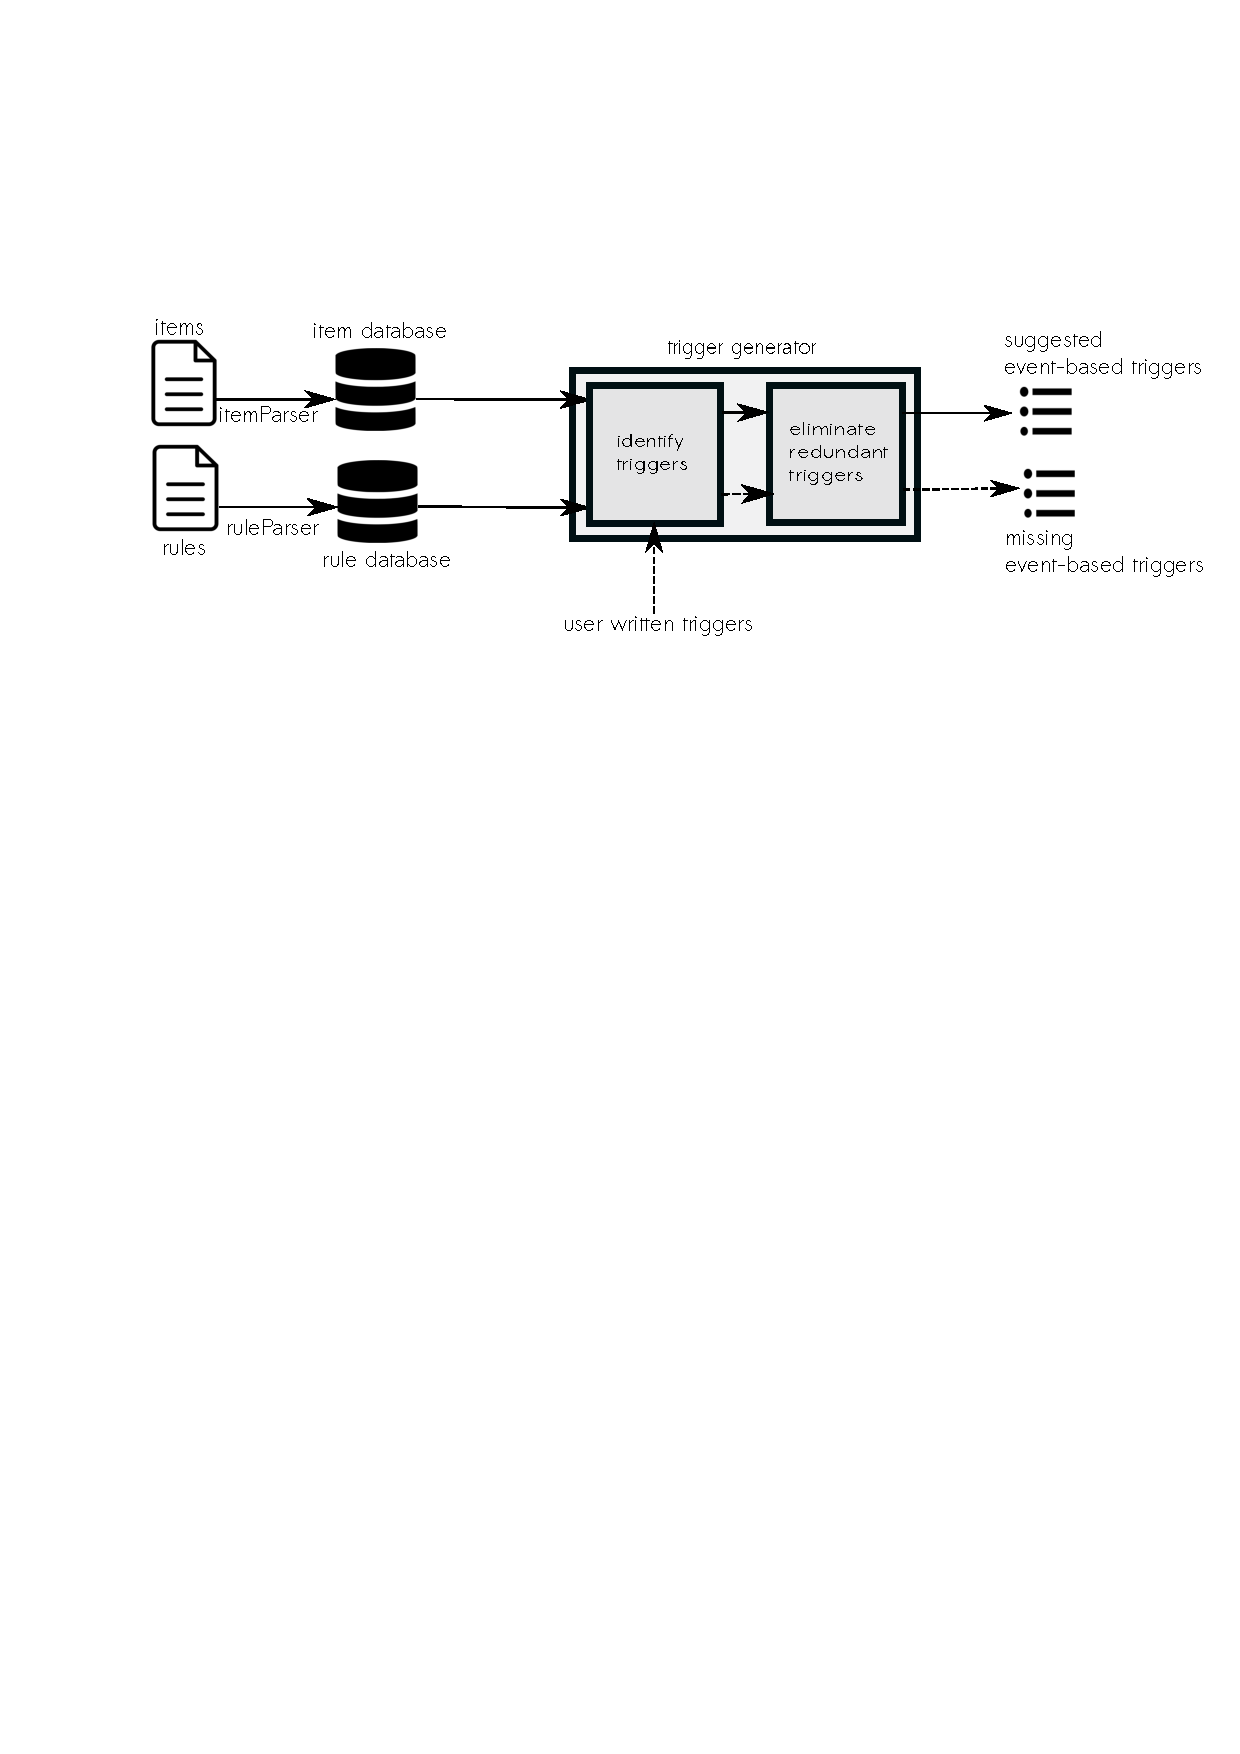
\includegraphics [trim=2cm 19cm 0 5.5cm, scale=0.45]{images/design.pdf}
\caption{Design of trigger generator tool.}
\label{fig:design}
\end{figure} 
 
\section{Experimental Results}
We evaluated our tool on 116 end user written rules. We obtained the rules from links provided on the openHAB website~\cite{data1},\cite{data2}. It took $\sim$ 7.12 ms for the tool to generate the triggers and find the missing triggers for all the rules. For 105 rules, our tool suggested a list of all required event-based triggers and for 77 rules, our tool found missing triggers when some triggers were already provide by the users. For 18 rules, our tool detected potential conflicts among one or more rules. 

\section{Conclusions}
Not surprisingly, our research shows that end user written rules \textit{are} often incorrect. We observed that a common error made by end users while writing the rules is having insufficient number of triggers, leading to fewer firings of the rules than necessary. To prevent this problem, we developed a tool that can automatically generate trigger conditions based on the actions in a rule as well as identify missing triggers if some of them are already provided. This reduces the burden of the end users by assisting them in including all the required triggers. \\
\emph{Scope.} While our tool is capable of generating all event-based triggers it cannot generate temporal triggers. This is because it runs directly on the rules without any additional annotations from the end users about their preferences and without that, it is impossible to infer the exact temporal triggers the user expects. 

\bibliographystyle{abbrv}
\bibliography{sigproc}  

\end{document}
